% Author: Matthew Turner

\documentclass[11pt,letterpaper]{article}
% \documentclass[11pt]{report}
% \documentclass{report}
% \documentclass{book}
\usepackage[bookmarks]{hyperref}
\usepackage{amssymb,amsmath}
% \usepackage{fullpage}
\usepackage{tabulary}
\usepackage{tabularx}
\usepackage{float}
% \usepackage[margin=1.00in]{geometry}
\usepackage[margin=0.90in]{geometry}

\usepackage{colortbl}
\usepackage[table]{xcolor}
\usepackage{caption}
\usepackage{booktabs}
\usepackage{pslatex}
\usepackage{apacite}
\usepackage{subcaption}
\usepackage{pgfplots}
\usepackage{wrapfig}
\usepackage[english]{babel}
\usepackage{lmodern}
\usepackage{setspace}
\doublespace
% \usepackage{url}
\usepackage{bigfoot}
\usepackage[export]{adjustbox}
\setlength\intextsep{0pt}

\usepackage{graphicx}

\title{Potential errors of sign and magnitude in behavioral studies of group polarization}

\author{{Matthew A.~Turner}}

\begin{document}
\maketitle

\begin{abstract}
  ``Group polarization'' is understood as a key social structuring process
  that increases extremism and exacerbates society-level polarization. 
  In group polarization,
  isolated groups similar in their biases on some topic become more extremely biased after
  deliberation. In order to understand the causes of group polarization, it is 
  necessary to perform behavioral studies to understand what sorts of groups
  do go to extremes in which situations. However, following the published
  behavioral studies would lead one to use statistical methods that are known
  to cause errors of magnitude and sign in determining effect sizes. 
  In general, unless one has knowledge of the variances of measurements it is
  impossible to know if there has been a false inference. In many cases
  the variance of data were not reported in original studies and are now
  lost to time. Must we conclude many published results are unreliable? 
  This paper shows that we can cautiously accept the results. We support
  this claim with computational experiments that recreate three case studies
  we use to understand the effects of using metric models on ordinal data
  in the group polarization setting specifically. We close by discussing the
  effect these findings have on the state of knowledge about group polarization
  and social structuring more generally, and whether more complicated ordinal
  models are really needed over the simpler, easier-to-understand
  metric models.
\end{abstract}


\section{Introduction}

Problem:
\begin{enumerate}
  \item
    Is there really evidence for group polarization as a general phenomenon?
    \begin{itemize}
      \item 
        This question arises due to several existing, commonly-referenced
        studies using metric
        statistical models to make inferences with ordinal data, which leads
        to false inferences in certain situations~\cite{Liddell2018}.
    \end{itemize}
\end{enumerate}

We will now introduce the group polarization
phenomenon, theoretical explanations, and review supporting evidence for
group polarization. Then we will
brielfy introduce how our model of statistical inference for group 
polarization may result in false inferences~\cite{Liddell2018}. In our
Results we will then apply this model three case studies taken from the
group polarization literature that use metric models with ordinal data.
Through simulations using published data and some knowledge about the
group polarization study procedures we will determine whether or not
results from these individual case studies must be rejected due to 
potentially false inferences.

\subsection{Group polarization studies not affected by this problem}

The group polarization effect is considered robust. The theory of group polarization has had
broader impacts beyond social psychology, notably on political psychology
and law~\cite{Sunstein2002,Sunstein2009,Sunstein2019}. Whether or not the 
published behavioral studies we analyze here using metric models on 
ordinal data make false inferences,  there are several alternative approaches
to group polarization experimental design. I explain some here to help us
better understand what group polarization is and explaining how the 
published empirical studies under investigation here fit within the broader
scope of group polarization studies.

\begin{itemize}
  \item Gambling studies where opinions are about how much risk is 
    acceptable \cite{Blascovich1973,Blascovich1974,Blascovich1975,Blascovich1975a,Blascovich1976}
  \item Pattern-oriented approach of \citeA{Mas2013} to demonstrate their
    model predicted general patterns of observed opinion dynamics.
  \item Jury deliberations about how much money to reward plaintiffs
    \cite{Myers1976,Kaplan1977,Schkade2000}.
\end{itemize}

\subsection{Group opinion polarization experiment design}

\begin{enumerate}
  \item
    (INTRO PAR) In this paper we develop a model of group opinion shift measurement,
    detection, and quantification based on experimental design in the literature.
    To motivate our model development, here we identify a common set of
    design elements used in group opinion polarization experiments and 
    provide some examples of how existing studies vary this basic design in
    order to answer specific theoretical questions about group polarization.
    \begin{itemize}
      \item 
        There are some basic, common elements among opinion-based group polarization
        which together we call the ``basic experimental paradigm'' for reference.
        In details, opinion-based group polarization experiments can vary greatly
        as needed for testing specific hypotheses.
      \item 
        No matter the research question, the basic outcome measure is the 
        group opinion shift before and after discussion. There are various ways
        to perform the measurements of individual opinions, but all 
        group polarization studies must measure a group opinion shift. 
        In group polarization studies, several group shifts are observed, so 
        the statistical tests to quantify the magnitude and sign of choice shift
        compare the pre-discussion and post-discussion opinion distributions.
      \item
        In the Model section below we explain in more detail methodologies
        for quantifying this shift. For now we focus on reviewing existing
        approaches to experimental design for inducing group opinion shifts.
      \item
        To give an illustrative example with historical relevance, we will use
        examples of how the research question and hypotheses have guided
        experimental design. These experiments were designed
        to determine the extent to which
        group opinion polarization occurs due to either 
        ``social comparisons''~\cite{Myers1978} or ``persuasive 
        arguments''~\cite{Vinokur1978}, 
        or in some combination of the 
        two~\cite{Burnstein1973,Burnstein1977,Sieber2019}.
    \end{itemize}
  \item 
    (THE BASIC EXPERIMENTAL PARADIGM---can still use examples, but focus
    only on the high level)
  \item 
    (OVERVIEW OF VARIATIONS AND THEIR PURPOSE---eg separating social comparisons
    from persuasive arguments requires an argument-free condition; explain 
    how those work so the reader understands the scope of the model)
\end{enumerate}




\subsection{Scope and limitations of this work}
  \begin{itemize}
    \item
      It is an important question exactly \emph{how} group polarization
      emerges~\cite{Sunstein2009,Turner2020}, 
      however that is irrelevant for this study. All that matters is 
    \item
      This study focuses on the specific problems that may occur when
      one makes statistical inferences using a metric data model with 
      ordinal data. There may be other problems with standard stastical
      practice in group polarization experiments. One important one may be
      the pooling of groups together based on initial bias, but not allowing
      for the random effect of group index that would lump together several
      other potential confounding factors that would be shared by each group
      such as weather or time of day that the experiment was administered~\cite{Clark1973,Baayen2008}.
      We explore these issues and how our model might be adapted to understand
      their effect on group polarization experiments in the Discussion.
  \end{itemize}


\section{Model and methods}

In this section we outline our general model of group polarization that focuses
on the measurement and inference procedures, and ignores the irrelevant
(for the purposes of this paper) factors of how opinions change. First in this
section we introduce our generic model of a group polarization experiment.
Then we introduce how we design our computational experiments to detect potential
false inference in published results. 
After introducing our modeling strategy in this section, we apply it
to three case studies in the next Analysis section.

\subsection{Model}
\begin{enumerate}
  \item Our model generalizes the group polarization experimental paradigm to 
    focus on measurement and inference. 
    
  \item 
    This model is agnostic regarding the cognitive, social, and
    communicative mechanisms that lead to group polarization.

  \item
    The group polarization experimental procedure has three main steps
    (Figure~\ref{fig:modelDiagram}).
    \begin{enumerate}
      \item 
        Form biased groups---methods for doing this vary, but our model
        is agnostic to how biased groups our formed because it is not relevant
        to evaluating the statistical procedure. We show how our model is
        appropriate in each of our case studies analyzed below. 
        (REVIEW METHODS BROADLY IN INTRO?)
      \item 
        Groups deliberate for a time $t_D$
    \end{enumerate}
\end{enumerate}

\begin{figure}
  \centering
  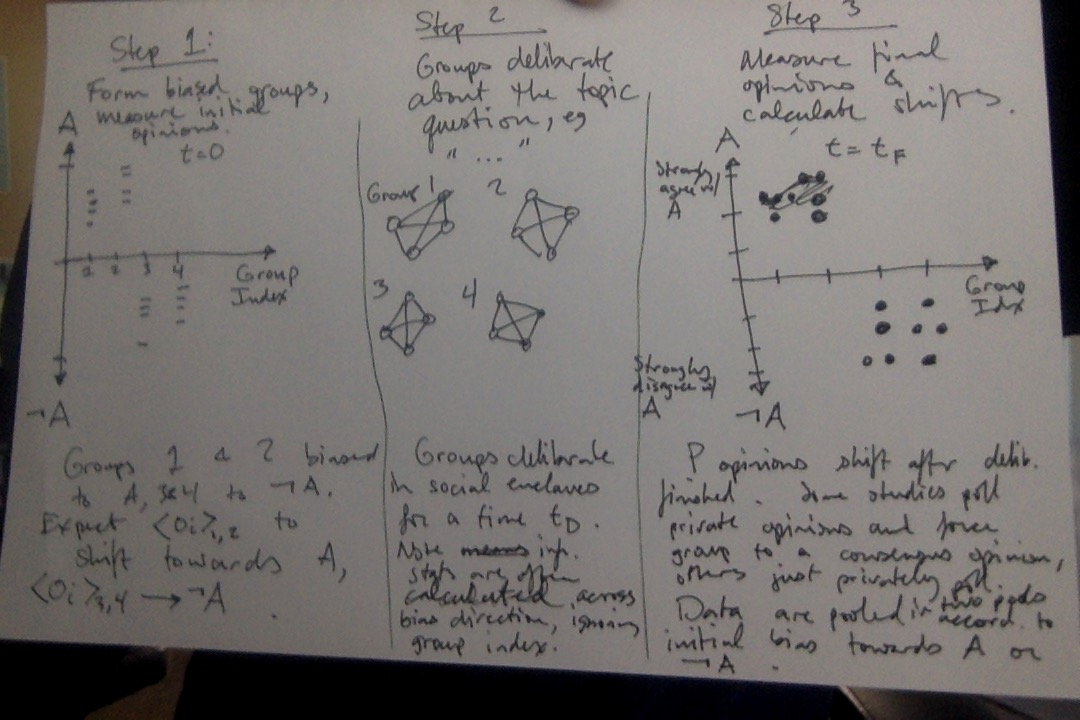
\includegraphics[width=0.7\textwidth]{Figures/ModelDiagramSketch.jpg}
  \caption{A data-centric model of a generic group polarization experiment.}
  \label{fig:modelDiagram}
\end{figure}
\subsubsection{Detecting false inference}

\begin{itemize}
  \item 
    The presence of the group polarization effect is calculated
    by applying inferential statistics, such as calculating Cohen's $d$, to
    determine whether the pre- and post-deliberation opinions changed
    (Figure~\ref{fig:falseInferenceDiagram}).
  \item
    It would be a false detection of the effect if, in fact, the latent pre- and
    post-deliberation means were equal, but a metric model (like Choen's $d$
    procedure) leads to the inference that means changed significantly. 
    This happens for certain combinations of the 
    variance of pre- and post-deliberation opinion distributions and the
    measurement strategy that converts latent opinions into reported, discrete
    opinions.
  \item
    (REVIEW GENERAL EXAMPLE FROM~\cite{Liddell2018})
\end{itemize}

\begin{figure}
  \centering
  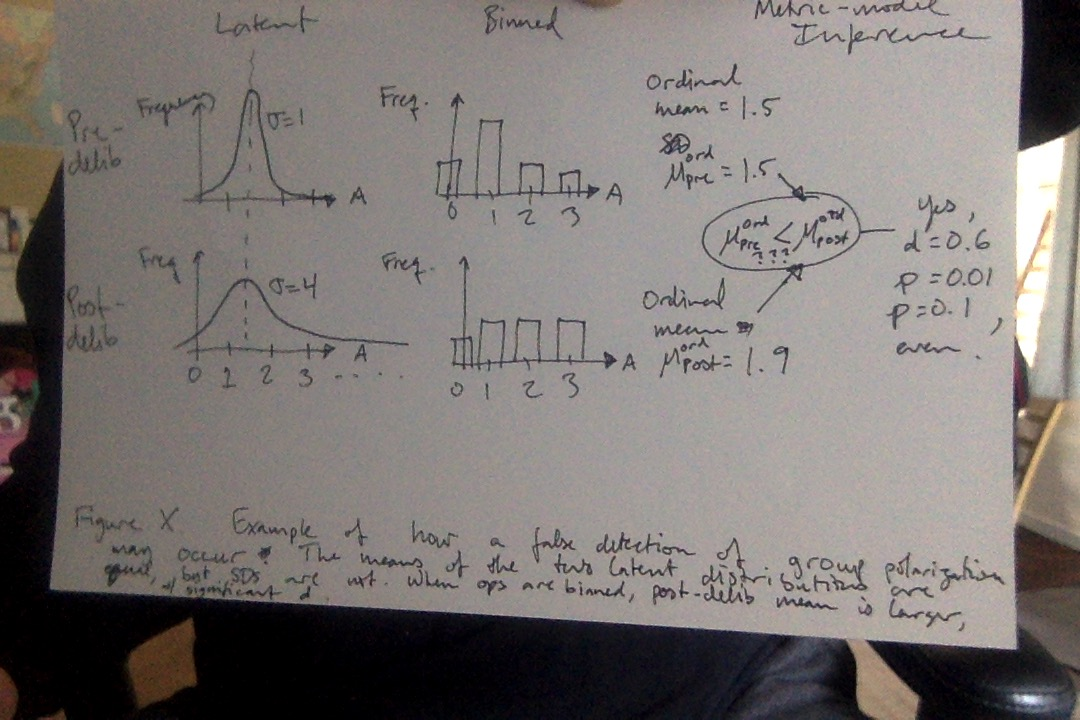
\includegraphics[width=0.7\textwidth]{Figures/FalseInferenceDiagram.jpg}

  \caption{Example of a false detection of group polarization under specific
  conditions. This requires the standard deviations of the latent opinion
  distributions to be different, with the post-deliberation variance greater
  than the pre-deliberation variance. As we will demonstrate, it is rare that
  this occurs in group polarization experiments, allowing us to cautiously accept
  published results.}\label{fig:falseInferenceDiagram}
\end{figure}

\subsection{Case study strategy}
(EXPLAIN HOW CASE STUDIES WILL HELP US TO KNOW HOW CONFIDENT WE CAN BE THAT
THE GROUP POLARIZATION EFFECT IS NOT BULLSHIT)
\begin{itemize}
  \item 
    Group polarization studies report the initial and final means of initially
    biased groups, at the least. 
  \item
    We try to induce a false group polarization effect by the following steps.
    If no group polarization effect is found, this is evidence that the
    reported effect is not a false positive. 
    \begin{enumerate}
      \item 
        We take the initial reported mean and use that as the initial latent
        group mean opinion. 
      \item
        We set the post-deliberation latent mean to be equal to the 
        pre-deliberation latent mean.
      \item
        If the standard deviations of opinion are given pre- and post-discussion, 
        these are used as if they were the standard deviation of the latent 
        distribution. If they are not given, we test a set of plausible 
        standard deviation values (WILL HAVE TO JUSTIFY WHICH ARE PLAUSIBLE)
      \item
        We take samples from the latent opinion distributions specified
        by pre- and post-deliberation mean and standard deviations, bin them,
        and take these as the measured opinions reported by (model)
        study participants. 
      \item
        We then use a metric two-tailed test to calculate Cohen's $d$ to detect
        a group polarization effect of increased group extremity, i.e. increased
        magnitude of the mean group opinion, following deliberation.
      \item
        If $d$ and $p$ are in the ``significant''  range, 
        we conclude a false inference is likely for the
        given distribution parameters and measurement strategy. If this 
        matches the distributions and measurement strategies in published
        results, then we must suspect that the published results contain
        misleading finding of the group polarization effect.
    \end{enumerate}
\end{itemize}

\section{Analysis}

We take a case study approach, selecting three high profile studies in the
group polarization associated social/political science 
literature~\cite{Sunstein2009,Sunstein2019}. While each implements the general
group polarization experimental model outlined above, they do it in different
ways, from the assembly of groups with aligned attitudes to the reporting and
analysis of collected research data. The approach of each case study is
outlined within the following subsections, each devoted to one of the three
case studies. For convenience the three case studies are summarized in
Table~\ref{tab:caseStudiesSummary}.

\vspace{2em}
\begin{table}[h]
  \rowcolors{2}{gray!25}{white}
  \centering
  \begin{tabular}{p{1in}p{1.25in}p{1.15in}p{1.5in}p{1.25in}}
    \rowcolor{gray!50}
    Reference  &  Topics   &  Group formation  & Opinion measurement  & Shift measurement  \\ \toprule
    Schkade, et al., (2010) & Global warming, affirmative action, civil unions
                            & 63 adults; one (US) ``liberal'', one 
                              ``conservative'' group
                            & 10-point Likert-style  
                            & F-tests reporting $t$ value \\
    Myers \& Bishop (1970) & Racial attitudes &  Pre-screened 
                                                 high school students 
                           & 18-point Likert-style scale  
                           & ANOVA (F and t tests)  \\
    Moscovici \& Zavalloni (1969) & French \& international politics
                                  & 140 graduating lyc\'{e}e students (18-19 yo)
                                  & 7-point Likert scale
                                  & $t$ test and Walsh test
                            
  \end{tabular}
  \caption{Summary of case studies analyzed below. The ``Shift measurement'' column lists the method used for measuring the group polarization opinion shift. One \href{http://www.statistics4u.com/fundstat_eng/ee_walsh_outliertest.html}{Googled reference} says Walsh requires $n > 220$, which the Moscovici and Zavalloni study does not meet.}
\end{table}

\begin{itemize}
  \item 
    We now turn to answer whether evidence for group polarization is reliable
    or not using our computational model.
  \item
    Recall our model assumes that each participant holds some latent ``internal'' opinion
    drawn from a continuous normal distribution. Each participant reports 
    their opinion on a Likert-type ordinal scale. 
  \item
    Because there are many studies demonstrating the group polarization effect
    using ordinal data, we do not evaluate each one. Instead we selected 
    three influential examples: two studies administered in the United States
    from two different decades, the 1960s and 2000s, and one administered in 
    France in the 1960s.
  \item
    We find that changes in variance between pre- and post-discussion opinions
    are important in determining whether or not published inferences are reliable.
  \item
    One of our case studies, the one from the US in 2010, does report variances,
    which enables us to confidently determine that it contains no false inferences.
  \item
    The other two case studies, and the vast majority of group polarization
    studies, do not report variance in pre- and post-discussion opinions.
    Still, due to widely accepted theories of consensus formation, variance
    in participant opinions decreases from pre- to post-discussion, which 
    enables us to cautiously accept that evidence does indeed exist to support
    the group polarization phenomenon in general.
\end{itemize}

\subsection{Case study I: A tale of two cities in Colorado, USA, in 2010}


  \begin{itemize}
    \item 
      \citeA{Schkade2010} sought to evaluate whether group 
      polarization occurs symmetrically in conservative and liberal groups.
      In other words, do ideological conservative and liberal groups both
      shift opinions following deliberation? Are the shift magnitudes 
      approximately the same, or does one group shift more?
    \item
      This question is important since in the US conservative and liberal
      groups increasingly accuse one another of inappropriate and
      dangerous extremism.
    \item
      \citeA{Schkade2010} recruited groups of six participants from
      two different cities in the state of Colorado, USA, in 2005. One city,
      Colorado Springs, is predominantly conservative, with about (TWO THIRDS?)
      voting for George W. Bush in the 2004 presidential election. The other,
      Boulder, had about (TWO THIRDS?) of its residents vote for John Kerry
      in the 2004 presidential election. 
  \end{itemize}
      
  \subsection{Experimental design in Schkade, et al., (2010)}
    (participant pool, survey questions,
    methodology---measurement and analysis)

    \begin{itemize}
      \item 
        Groups gave their opinions, discussed, then gave opinions again on
        three questions on current topics of political debate.
      \item
        THE QUESTIONS
      \item
        MEASUREMENT SCALE
      \item
        STATISTICAL PROCEDURES
    \end{itemize}
    \subsection{Study data and conclusions in Schkade, et al., (2010)}
    \begin{itemize}
      \item 
        Groups from both cities became more extreme following group discussion.
      \item
        Conservatives were found to shift more, but possiby due to liberals 
        starting with more extreme positions. CHECK WHETHER OUR MODEL CAN
        SHOW A FALSE POSITIVE ON GREATER CONSERVATIVE SHIFT---THIS WOULD ALSO BE
        CONTRARY TO THE ASSERTION THAT CONSERVATIVES ARE LESS OPEN AND AGREEABLE.
    \end{itemize}

\subsection{Analysis}

\begin{itemize}
  \item
    We found that reduction in variance after deliberation can plausibly explain observed
    group polarization opinion shifts in half of the experimental conditions
    used by Schkade and co-authors.
    \begin{itemize}
      \item 
        In three of the six experimental conditions (two ideologies x three
        deliberation topics) we can generate observed shifts simply by changing
        the variance, not the mean, between pre- and post-deliberation 
        opinions. 
      \item
        Furthermore, a range of latent opinion means and pre- and post-deliberation
        variances generate can generate opinion distributions with the reported
        values. The frequency of generating observed parameters is shown in 
        Figure~\ref{fig:successHeatmaps} (TODO). This indicates the range of plausible
        latent variances assuming no change in latent mean following deliberation.
        While there is a range of latent means that generate Schkade and 
        co-authors' research data, we present one that worked particularly
        well, found informal R command-line trial and error. Our analysis script and 
        associated notebook are provided in the GitHub repository for this
        project and in the supplement, respectively. The interested reader can
        easily run our script with different latent means to observe its effect.
      \item
        We were able to generate data with identical parameters reported in
        the paper over a range of plausible latent distribution parameters. 
      \item
        We generated false positives in 
        two conditions from the
        Boulder group and one condition from the Colorado Springs group.
      \item
        To do this we identified a latent mean
        and pre- and post-deliberation variances that lead to the observed
        shift when the model participants' latent means are reported (binned)
        on this study's 10-point Likert scale. These means and variances are
        listed below for each of the three false positives we generated.
    \end{itemize}
  \item 
    These findings suggest that group polarization mechanisms are not active,
    but only consensus mechanisms.
  \item
    Apparently, Schkade and coauthors take the numbers in Table 1 (geographical
    group-level shift on each question, with number of participants who increased,
    stayed the same, and decreased) to support their conclusion that 
    group polarization was occurring on all deliberation topics. All 
    significance tests contained in the paper
    were to determine whether Boulder (liberal) and Colorado Springs
    (conservative) opinion distributions differed initially, and that the
    shifts in city group were in opposite directions, with different magnitudes.
    No statistical inference was performed to quantify the evidence that exists
    for concluding that group polarization was active in all experimental conditions.
    When we performed significance testing \emph{on the simulated experimental data},
    the results were found to be insignificant in the three false positive
    cases we identified! This suggests the possibility that significance tests
    of ``ideological amplification'' were not included because they were not
    supportive of the paper's conclusions.
\end{itemize}
\begin{figure}
  \centering
  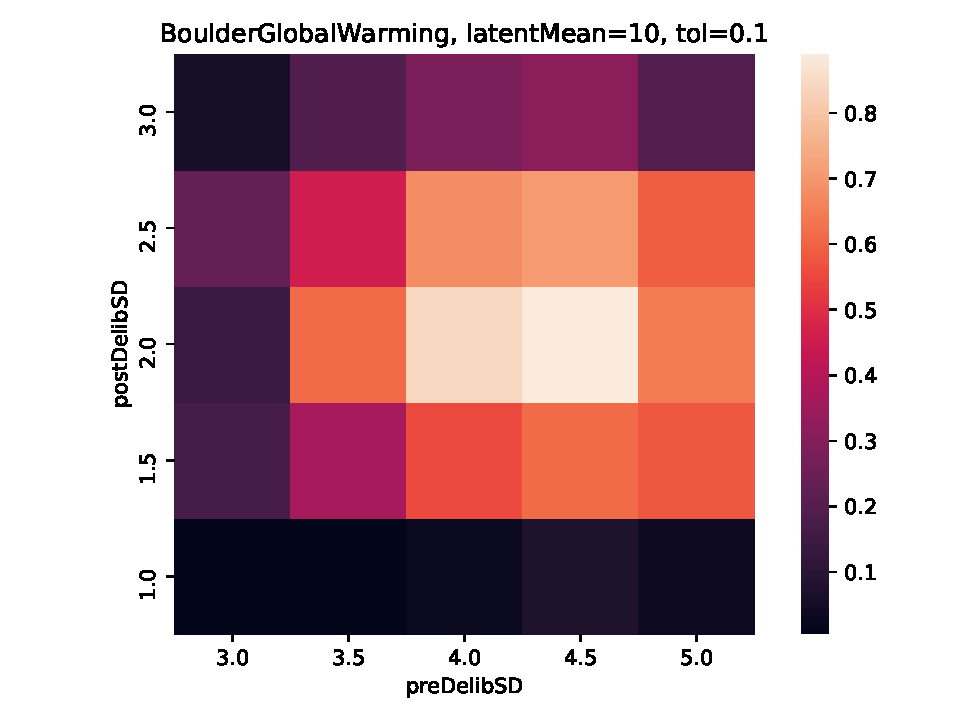
\includegraphics[width=\textwidth]{{Figures/Schkade2010/BoulderGlobalWarming_latentMean=10_tol=0.1}.pdf}
  \caption{Success rate of recreating reported group opinions and opinion
  shifts for different latent parameter combinations. Further parameter
  combination examples---lower tolerance and other latent mean---are (WILL BE) given in
the supplement.}
  \label{fig:successHeatmaps}
\end{figure}


% \begin{table}[h]
%   \centering
%   \begin{tabular}{cccc}
%     Site  &   Topic  &   Pre-delib mean  &  Post-delib mean  &  FP Latent Mean   \\
%       \toprule
%     Boulder  &   Global warming  & 9.19 & 9.44 & 9.98  \\
%     Boulder  &   Civil unions    & 9.22 & 9.69 & 10
%     Colorado Springs  &   Civil unions    & 
%   \end{tabular}
% \end{table}



\subsection{Case study II: French attitudes about their president and Americans}

\citeA{Moscovici1969}


\subsection{Case study III: Racial attitudes in the USA in the late 1960s}

\citeA{Myers1970}

\section{Discussion}

\begin{itemize}
  \item 
    In this paper we developed a computational statistical model of group
    polarization to better understand how psychological theory and statistical 
    procedures could affect measurements and estimates of group polarization. 
  \item
    We put this understanding to 
    practical use. First, we re-evaluated existing published results, providing our
    method that could be used to re-evaluate other group polarization results,
    or results from other fields using similar measurement and statistical
    procedures. Then we prescribed a more robust statistical procedure that should
    be used in group polarization studies, or any other study that is measuring
    changes in some theoretical psychological entity such as ``opinions'' using
    a discrete reporting scale, such as a Likert scale.
  \item
    Our analysis did not consider the separate, but important, issue about
    the causes of group polarization. We hope Our analysis does suggest that 
    scrutiny of opinion dynamics at the extremes could be valuable.
    Our updated look at 
    published results reveals that group polarization findings do seem to be
    legitimate when opinions are not too extreme. However, on issues where
    opinions are more extreme to begin with, extremity may not increase 
    nearly as much as variance in opinion decreases. 
    A theoretical question with practical importance, then, regards the
    nature of opinions themselves: do they vary continuously? Can they increase
    without limit, or do they have an upper bound? What is the connection 
    between the opinion reported by a participant and neurobiological 
    activity, and how can a better understanding of neurobiology improve
    models of group- and society-level behavior? 
  \item
    When we took a close look at common measurement and statistical procedures
    used in the group polarization literature, we noticed an additional problem: 
    many obvious sources of variance are excluded from the statistical analysis.
    Group polarization studies are but one of several fields that struggle
    with including relevant sources of variance in their statistical models~\cite{Yarkoni2021}.
    In the case of group polarization, one could infer from similar models
    that if group- and individual-level variation were included in the
    statistical model, . It could be valuable in future work, then, to 
    develop a statistical model of how multilevel statistical modeling could
    affect group polarizaiton results, then combine that analysis with the
    analysis of the present paper regarding measurement and inference.
\end{itemize}

% Make sure to RePAV your paper often. That is, check on how well you have
% stated
% \begin{enumerate}
%   \item \textbf{Re}search tradition/community you are addressing
%   \item \textbf{P}roblem you are addressing/solving
%   \item \textbf{A}pproach taken
%   \item \textbf{V}alue of the work
% \end{enumerate}

\bibliographystyle{apacite}

\setlength{\bibleftmargin}{.125in}
\setlength{\bibindent}{-\bibleftmargin}

\bibliography{/Users/mt/workspace/papers/library.bib}

\end{document}
